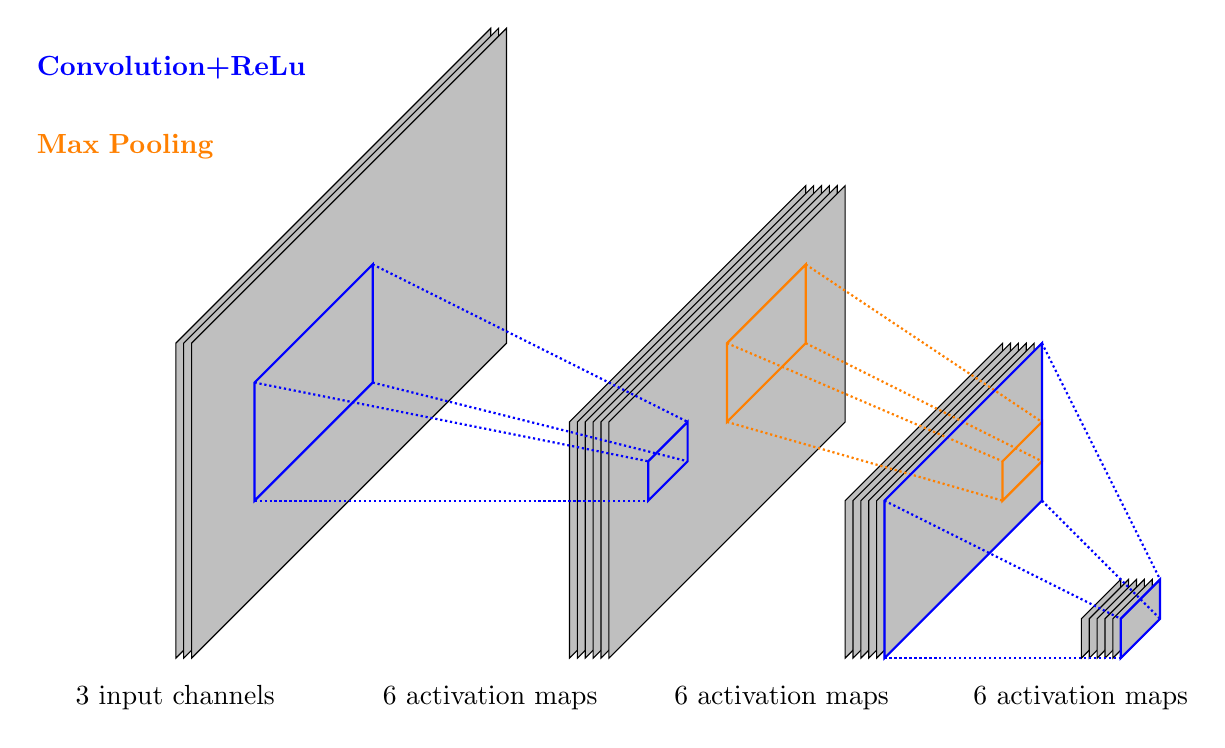
\begin{tikzpicture}
	\begin{scope}[yslant=1,xshift=0.2]
		\foreach \i in {0,0.1,0.2}
			\draw [fill=lightgray] (0+\i,0-\i) rectangle (4+\i,4-\i);
		
		\foreach \i in {0,0.1,0.2,0.3,0.4,0.5}
			\draw [fill=lightgray] (5+\i,-5-\i) rectangle (8+\i,-2-\i);
			
		\foreach \i in {0,0.1,0.2,0.3,0.4,0.5}
			\draw [fill=lightgray] (8.5+\i,-8.5-\i) rectangle (10.5+\i,-6.5-\i);
			
		\foreach \i in {0,0.1,0.2,0.3,0.4,0.5}
			\draw [fill=lightgray] (11.5+\i,-11.5-\i) rectangle (12+\i,-11-\i);
		
		\draw [thick, blue] (1,1) rectangle (2.5,2.5);
		\draw [thick, blue] (6,-4) rectangle (6.5,-3.5);
		\draw[densely dotted, blue, thick] (1,1) -- (6,-4);
		\draw[densely dotted, blue, thick] (1,2.5) -- (6,-3.5);
		\draw[densely dotted, blue, thick] (2.5,1) -- (6.5,-4);
		\draw[densely dotted, blue, thick] (2.5,2.5) -- (6.5,-3.5);
		
		\draw [thick, orange] (7,-4) rectangle (8,-3);
		\draw [thick, orange] (10.5,-8) rectangle (11,-8.5);
		\draw[densely dotted, orange, thick] (7,-4) -- (10.5,-8.5);
		\draw[densely dotted, orange, thick] (7,-3) -- (10.5,-8);
		\draw[densely dotted, orange, thick] (8,-4) -- (11,-8.5);
		\draw[densely dotted, orange, thick] (8,-3) -- (11,-8);
		
		\draw [thick, blue] (9,-9) rectangle (11,-7);
		\draw [thick, blue] (12,-12) rectangle (12.5,-11.5);
		\draw[densely dotted, blue, thick] (9,-9) -- (12,-12);
		\draw[densely dotted, blue, thick] (9,-7) -- (12,-11.5);
		\draw[densely dotted, blue, thick] (11,-9) -- (12.5,-12);
		\draw[densely dotted, blue, thick] (11,-7) -- (12.5,-11.5);
	\end{scope}
	
	\node (in) at (0,-0.5) {3 input channels};
	\node (h1) at (4,-0.5) {6 activation maps};
	\node (h2) at (7.7,-0.5) {6 activation maps};
	\node (out) at (11.5,-0.5) {6 activation maps};
	
	\node [text=blue, align=left,text width=10em] (conv) at (0,7.5) {\bf Convolution+ReLu};
	\node [text=orange, align=left,text width=10em] (pool) at (0,6.5) {\bf Max Pooling};
\end{tikzpicture}